\documentclass[a4paper]{article}

%% Language and font encodings
\usepackage[english]{babel}
\usepackage[utf8x]{inputenc}
\usepackage[T1]{fontenc}

%% Sets page size and margins
\usepackage[a4paper,top=3cm,bottom=2cm,left=3cm,right=3cm,marginparwidth=1.75cm]{geometry}

%% Useful packages
\usepackage{amsthm}
\usepackage{amsmath}
\usepackage{amssymb}
\usepackage{graphicx}
\usepackage[colorinlistoftodos]{todonotes}
\usepackage[colorlinks=true, allcolors=blue]{hyperref}
\usepackage{mathabx}
\usepackage{tikz}

\setlength\parindent{0pt}

\title{CS 4780/5780 Homework 2}
\author{Due: Tuesday 09/25/18 11:55pm on Gradescope}
\date{}

\begin{document}
\maketitle

The following problems concern the perceptron. Using the knowledge you learned in class about when the perceptron may be applied, we will analyze how to algorithmically train the perceptron, and determine when the perceptron converges.



\subsection*{Problem 1}
% Learning goals: algorithm familiarity and algebra.
You are preparing for a competition on using the perceptron algorithm \textit{without computational aid}. Consider the following two-point 2D dataset:
\begin{enumerate}
	\item Positive class (+1): $(1, 3)$
	\item Negative class (-1): $(-1, 4)$
\end{enumerate}
Starting with $w_0=(0,0)$, how many updates will you have to perform to $w$ until convergence? Write down the sequence of each updated $w_i$ ([$w_1,w_2...w_n$]) by iterating the data points in the order: $[(1, 3), (-1, 4)]$.

\subsection*{Problem 2}
% Learning goals: perceptron prediction formula, error formula for perceptrons, training error is 0.
Suppose your boss Celeste gives you a fully trained (i.e. converged) Perceptron with weight vector $w$, the training set used to train it ($D_{TR}$), and a separate test set ($D_{TE}$). Here $x\in\mathbb{R}^d$ and $y\in\{-10,+10\}$. She wants to know whether the test error is greater than the training error. 

\subsubsection*{a)}
Your co-worker Klotilde says it will help to evaluate $h(x)=\text{sign}(w\cdot x)$ for every $(x,y)\in D_{TR}$ and every $(x,y)\in D_{TE}$. Does his suggestion help to determine whether the test error is higher than the training error? Why or why not? Please use the formula for error rate to explain your answer.

\subsubsection*{b)}
Can you determine whether the test error is greater than the training error, without looking at all of the points $D_{TR}$ and $D_{TE}$? If so, how? If not, why?

\subsection*{Problem 3}
% Learning goals: "margin" (as used in convergence proof) vs "minimum distance", upper bound on number of updates, linear separability requirement.
Your friend asks for your help on how to use the proof from class to find an upper bound for the convergence time of the perceptron algorithm. She gives you the following 3-point 2D dataset (See figure 1. Green = positive, Red = negative):
\begin{enumerate}
\item Positive class: $(-1, 1)$
\item Negative class: $(1,0)$, $(0,-1)$

\begin{figure}[h!]
	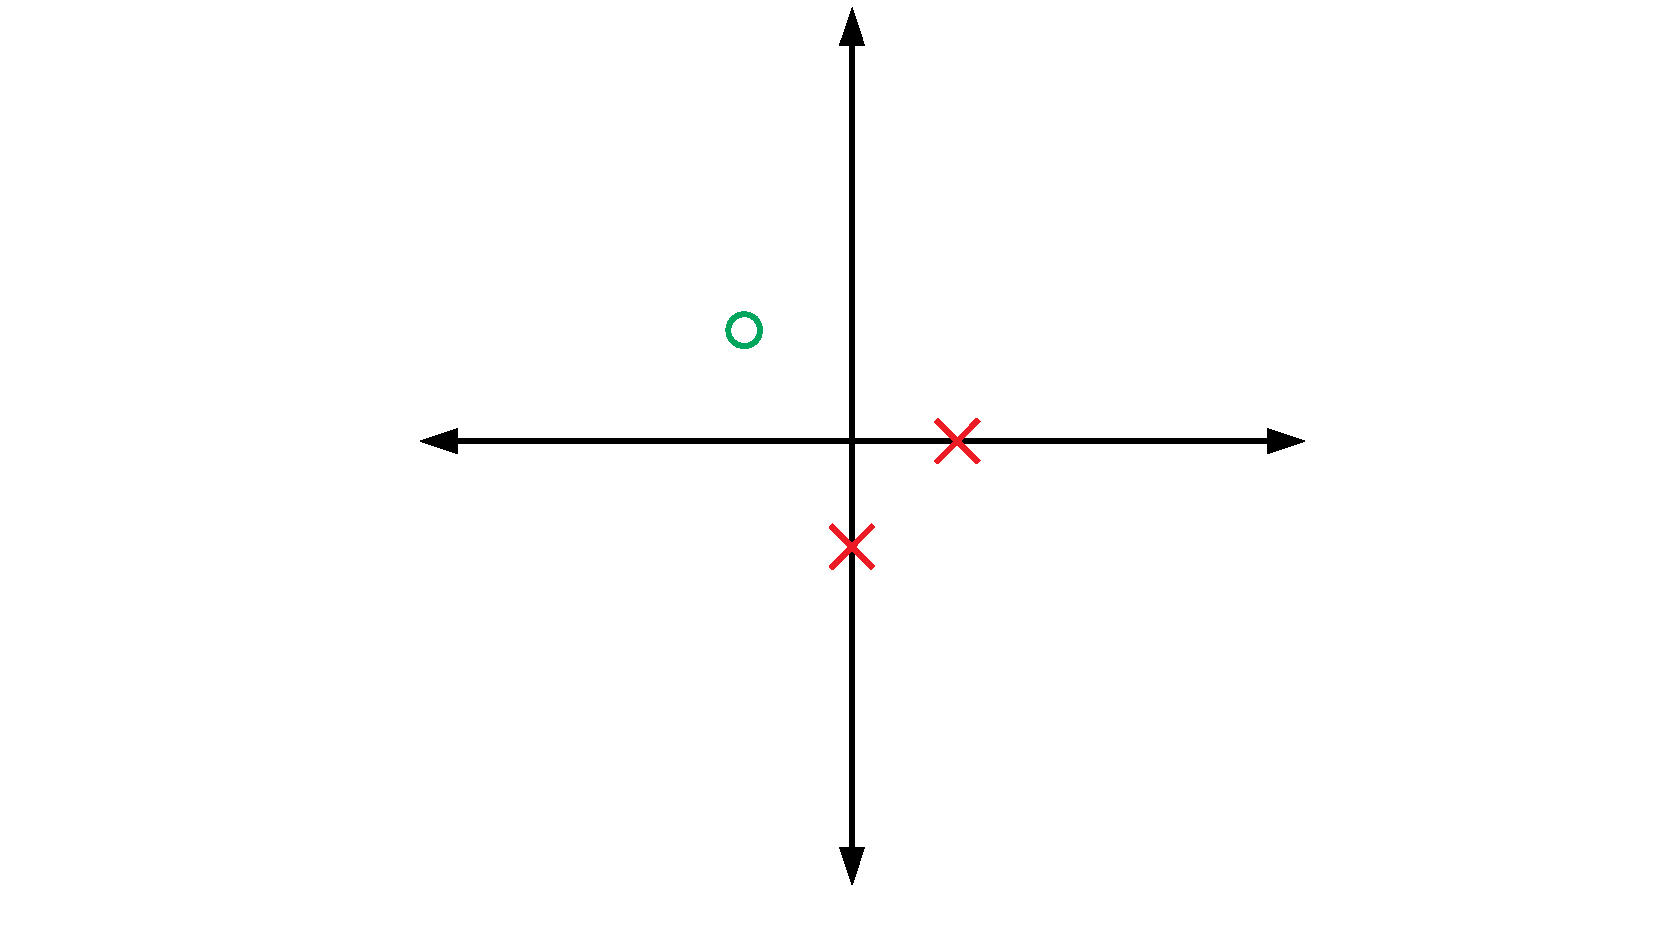
\includegraphics[width=10cm]{p3.pdf}
	\centering
	\caption{Illustration for Problem 3.}
\end{figure}
\end{enumerate}
\subsubsection*{a)}
What is the minimum distance between these points and the hyperplane defined by $w=(-1,1)$? Why is this \textit{not} the $\gamma$ defined in the proof?
\subsubsection*{b)}
Find a valid value of $\gamma$. Using the theorem from class, what is an upper bound on the number of updates the perceptron will make?
\subsubsection*{c)}
Chiku adds the point $(1,-1)$ to the positive class. What is the new upper bound on the number of updates the perceptron will make?

\subsection*{Problem 4}
% Learning goals: weight vector is linear combination of training dataset.
Your friend Cuneyt comes to you, desperate for your Perceptron expertise. His dataset is massive (with more than 10 trillion training examples), and after hours of training his perceptron (until convergence), his code malfunctioned and did not save the final weight vector.\\

Thankfully, at every training iteration, the code saved which example was used for the update step. Surprisingly, only five of the 10 trillion+ training examples were ever misclassified. They are listed below, along with the number of times they were used in an update step.

\begin{center}
\begin{tabular}{ c c }
 Training Example & Number of Times Used in an Update Step \\ 
 \hline
 (0, 0, 0, 0, 4),	+1 & 2  \\
 (0, 0, 6, 5, 0),	+1 & 1  \\
 (3, 0, 0, 0, 0),	-1 & 1  \\
 (0, 9, 3, 6, 0),	-1 & 1  \\ 
 (0, 1, 0, 2, 5),	-1 & 1     
\end{tabular}
\end{center}

What is the final weight vector of this perception (i.e. the weight vector that would have been saved if the code had not malfunctioned)?
















\end{document}
